\paragraph{Einleitung}\label{par:stft:intro}
%
Als erstes wollen wir uns mit der Fourier-Analyse von Signalen beschäftigen.
Hierbei ist das Ziel das Verhalten eines Signals im Frequenzbereich zu charakterisieren.
Wir wollen jedoch in unserer Analyse davon ausgehen, dass wir ein Signal $x[\cdot]$ vorliegen haben, dessen spektrale Eigenschaften \emph{zeitvariant} sind.
Hiermit ist \emph{nicht} gemeint, dass wir davon ausgehen, dass das Signal zeitvariant ist, denn das ist es natürlich.
Es geht darum, dass der Anteil der verschiedenen Frequenzen in einem Signal sich mit der Zeit ändert.
Natürlich ist hier eine der am einfachsten zugänglichen Anwendungen die Analyse von Audiosignalen.

Beginnen wir mit einer intuitiven Betrachtung.
Zunächst wollen wir einen möglichst großen Bereich im Frequenzbereich abdecken -- zumindest den für die jeweilige Anwendung relevanten.
Da sich beispielsweise im Audiobereich oft an der menschlichen Hörcharakteristik orientiert wird, die jenseits von \SI{20}{\kilo\hertz} nichts mehr leistet, sind Frequenzen jenseits dieser Grenze nicht mehr relevant.
Das heißt, dass sinnvollerweise ein Audiosignal mit einer Sample-Rate von \SI{40}{\kilo\hertz} bereits absolut ausreichend aufgenommen wurde.
Für andere Anwendungen lassen sich oft ähnliche Argumente finden, da die meisten physikalischen Systeme eine Tief- oder Bandpasscharakteristik \q{versteckt} haben, und man somit nur sehr selten mit Signalen mit immensen Bandbreiten konfrontiert ist.
Zusammenfassend muss also die Sample-Rate so angepasst werden, dass sie entsprechend unserer Anforderungen ausreicht.

Darüber hinaus ist uns aber auch gut daran getan, die Frequenzen, die in dem Signal vorkommen, sehr gut unterscheiden zu können.
Wir wollen also möglichst \emph{genau} wissen, welche einzelnen Frequenzen im Signal vorhanden sind. 
Das heißt, dass wir für eine tatsächlich im Signal vorhandene Frequenz $F$ aus unserer Analyse eine Frequenz erhalten wollen, die im Intervall $[F-\Delta_1,F+\Delta_1]$ für möglichst kleines $\Delta_1 > 0$ liegt.
In diesem Sinne wollen wir also möglichst große \emph{Auflösung}.
Wenn wir daran denken, dass $\Delta_1 = F_s/N$ gilt, so scheint es zu helfen, dass wir ein Signal möglichst lange \q{beobachten} müssen, also $N$ sehr groß wählen müssen.

Doch es gibt noch einen weiteren Auflösungsbegriff, der vom ersten strikt zu unterscheiden ist.
Wir wollen außerdem eine maximale Trennschärfe zwischen zwei unterschiedlichen Frequenzen, die gleichzeitig im Signal vorhanden sind, erreichen.
Wir wollen also in unserer Analyse zwei Frequenzen $F_1$ und $F_2$ mit $\Abs{F_1 - F_2} = \Delta_2$ immernoch unterscheiden und beider Existenz erkennen können.
Wiederum ist hier das minimale $\Delta_2 > 0$ von Interesse, für das diese Unterscheidbarkeit noch gilt, da dieses ein weiteres Auflösungslimit unseres Systems ist.
Ähnlich wie bei $\Delta_1$ ist auch hier der Beobachtungszeitraum $N$, welchen wir als Grundlage für unsere Analyse verwenden, von Bedeutung. 
Längere Zeiträume erlauben eine bessere Auflösung \emph{zwischen} Frequenzen.

Außerdem ist es noch oft interessant, dass man einen hohen Dynamikbereich abdecken kann.
Dies meint, dass man Frequenzanteile mit Frequenzen $F_1$ und $F_2$ und Amplituden $A_1$ und $A_2$ noch als zwei wahrnimmt, beziehungsweise beide noch erkennt, solange $\log(A_1/A_2) > \Delta_3$. 
Je größer das maximale $\Delta_3$ ist, desto besser, da prominente Frequenzanteile nicht weitere weniger stark ausgeprägte Anteile maskieren.

Schlussendlich haben wir es auch mit zeitvarianten Frequenzanteilen zu tun.
Das heißt, dass sich zum Zeitpunkt $T_1$ die Zusammensetzung der Frequenzen eines Signals $x$ von denen zum Zeitpunkt $T_2$ unterscheidet.
Für $\Abs{T_1 - T_2} > \Delta_4$ wollen wir also erkennen, dass $x[T_1]$ andere spektrale Charakteristik hat als $x[T_2]$ und die für möglichst kleine $\Delta_4$.
Diese zeitliche Evolution des Spektrums ist natürlich von immenser Bedeutung, weil man möglichst genau wissen möchte, \emph{wann} sich Frequenzen im Signal verändern.
Ideal wäre es also, wenn wir eine Art \q{instantane} Frequenzanalyse durchführen könnten, die trennscharf in einem infinitesimalen Intervall die jeweiligen Frequenzanteile aus dem Signal extrahiert.
Doch Schwingungen sind inhärent \emph{ausgedehnte} Effekte.
Ein kleines $\Delta_4$ steht also in direktem Widerspruch zu den Anforderungen an unsere Analyse für, gute (lies: kleine) $\Delta_1$ und $\Delta_2$, da wir dort gesehen haben, dass wir das Signal \emph{lange} beobachten müssen.
Für diesen Beobachtungszeitraum nehmen wir aber das Signal als \q{konstant} im Frequenzbereich -- also genau kontraproduktiv für ein kleines $\Delta_4$.
Dieser Widerspruch ergibt also eine Art Unschärferelation zwischen Frequenz-/ und Zeitauflösung.

Die zugehörige Transformation nennen wir \gls{stft}.
Wir wollen uns hier lediglich mit der diskreten Version der \gls{stft} befassen, weil wir diese uns als Analysetool von abgetasteten Daten vorstellen, die mit Rate $F_s$ aufgenommen wurden.
Uns liegt als das Signal $x: \R \rightarrow \C$ vor, das wir zum diskreten Signal $x[\cdot]$ abgetastet haben.
%
\paragraph{Definition}
%
Dann definieren wir eine Fensterbreite $W \in \N$ und eine Verzögerung $S \in \N$ und bilden die $W$-dimensionalen Vektoren $\bm x_s$ als
\[
\bm x^\ell_n = [x[\ell \cdot S + n]]_{n = 0}^{W-1} \in \C^{W}
\]
und mit diesen eine zweidimensionale Datenstruktur (keine Matrix!)
\[
\bm X = [\bm x^1, \ldots, \bm x^L] \in \C^{W \times L},
\]
welche aus $L$ vielen \q{Fenstern} in $x[\cdot]$ der Länge $W$ besteht.
Dann berechnen wir spaltenweise die \gls{dft} auf $\bm X$ und erhalten $\bm X_{\rm stft}$.
%
\paragraph{Interpretation} Im Licht der überlegungen aus \nameref{par:stft:intro} können wir nun diese Definition interpretieren und noch etwas aufbohren, um bessere Eigenschaften beziehungsweise mehr Information aus der \gls{stft} zu erhalten.
Dabei machen wir uns zunutze, dass eine diskrete \gls{stft} \q{nur} eine blockweise angewandte \gls{dft} ist.
Das heißt, dass deren Eigenschaften sich ausnutzen lassen, um die \gls{stft} zu beeinflussen.

Zunächst stellen wir fest, dass wir in einem Block von $\bm{X}_{\rm stft}$ eine Frequenzauflösung von $\Delta_1 = F_s / {N W}$ erhalten, da die Periodendauer eines Blockes im Zeitbereich die Länge ${WN}/F_s$ hat.
Jetzt könnte man auf die Idee kommen, dass man diese Auflösung verbessern will.
Eine Möglichkeit besteht darin die Fensterbreite künstlich zu verlängern.
Eine beliebte Herangehensweise ist an $\bm{X}$ eine bestimmte Anzahl von Nullen anzuhängen.

Dieses sogenannte \emph{zero-padding} wird in \Cref{py:stft_zp} gezeigt.
Man sieht, dass man bei Hinzufügen von $2N$ Nullen an ein Signal der Länge $N$ eine \emph{Interpolation} der \gls{dft} erreicht.
Diese Technik kann dann \q{blockweise} bei der \gls{stft} angewandt werden, um einen besseren Überblick des Spektrums zu bekommen.
Beispielsweise erlaubt dies auch eine genauere Bestimmung des Maximums der \gls{dft}, was der im Signal \q{prominentesten} Frequenz entspricht.
Da wir aber nur Nullen im Zeitbereich anhängen, entsteht keine neue Information, sondern wir erhalten nur zusätzliche Zwischenwerte.
Für die \gls{stft} heißt das, dass wir lediglich ein schöner aufgelöstes Bild erhalten, wenn wir zero-padding anwenden.
%
\begin{listing}[ht]
    \noindent
    \begin{minipage}{0.51\textwidth}
        \strut\vspace*{-\baselineskip}\newline
        \inputminted[firstline=4, lastline=20]{python3}{code/stft_zp.py}
    \end{minipage}%
    \begin{minipage}{0.48\textwidth}
        \strut\vspace*{-\baselineskip}\newline
        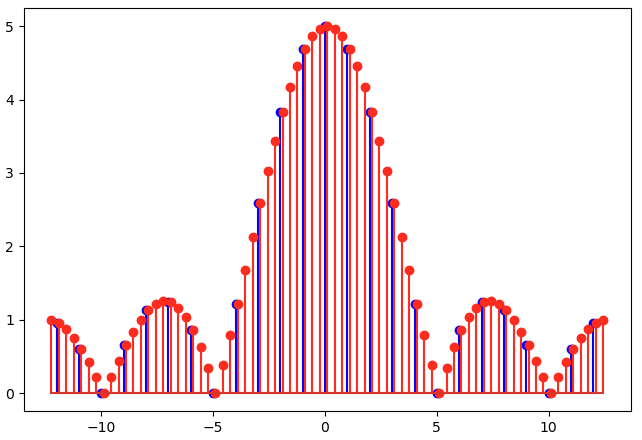
\includegraphics[width=\textwidth]{code/stft_zp.png}
    \end{minipage}
    \codecaption{dsv/code/stft_zp.py}{Zero-padding im Zeitbereich einer $\Rect$-Funktion liefert eine überabtastung der $\Sinc$-Funktion im Frequenzbereich}\label{py:stft_zp}
\end{listing}
%
%
\clearpage
Wir sehen auch noch einen weiteren Effekt von zero-padding, wenn wir ein harmonisches Signal mit der \gls{dft} analysieren.
Die \gls{ft} einer einzelnen Sinusschwingung mit Frequenz $F_0$ entspricht genau zwei komplexen Dirac-Stößen bei $\pm F_0$.
Doch was wir im Plot von \Cref{py:stft_harm} sehen ist, dass wir dies im Diskreten nicht reproduzieren können.
Bei Anwendung der Technik aus \Cref{py:stft_zp} stellt sich heraus, dass wir eher eine Faltung der Dirac-Stöße bei $\pm F_0$ mit einer (periodischen) $\Sinc$-Funktion sehen.
Deren Auftreten lässt sich dadurch erklären, dass zero-padding eines Signals der Länge $N$ auf Länge $M$ im Zeitbereich der Multiplikation eines Signals mit einem diskreten $\Rect$-Signal entspricht, welches bei $N$ vielen Werten den Wert $1$ annimmt, siehe \Cref{py:dft_1}.
Da dessen \gls{dft}, wie in \Cref{py:stft_zp} gezeigt, einem $\Sinc$ entspricht, sehen wir im Frequenzbereich die genannte Faltung.
Wenn wir im Zeitbereich die Länge des Signals auf $2N$ verlängern, so multiplizieren wir mit einer \q{breiteren} $\Rect$-Funktion im Zeitbereich und erhalten so einen \q{proportional schmaleren} $\Sinc$ im Frequenzbereich.

Für die \gls{stft} heißt das, genau das, was wir oben schon intuitiv analysiert haben. 
Beobachten wir das Signal in einem längeren Block, so können wir benachbarte Frequenzen besser auseinanderhalten.
Dies gilt jedoch nur, wenn sich diese Zusammensetzung im Frequenzbereich nicht stark ändert, während man diese Analyse durchführt, also innerhalb eines Blocks.
%
\begin{listing}[ht]
    \noindent
    \begin{minipage}{0.51\textwidth}
        \strut\vspace*{-\baselineskip}\newline
        \inputminted[firstline=4, lastline=19]{python3}{code/stft_harm.py}
    \end{minipage}%
    \begin{minipage}{0.48\textwidth}
        \strut\vspace*{-\baselineskip}\newline
        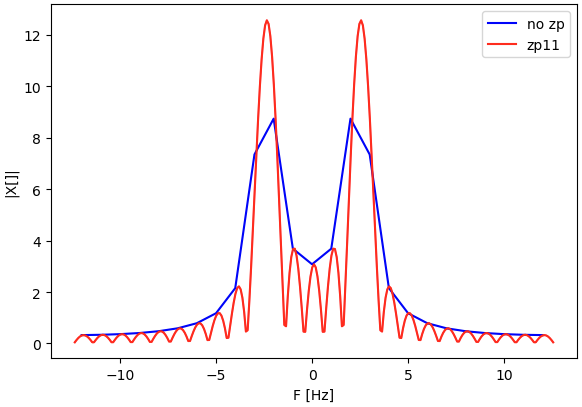
\includegraphics[width=\textwidth]{code/stft_harm.png}

        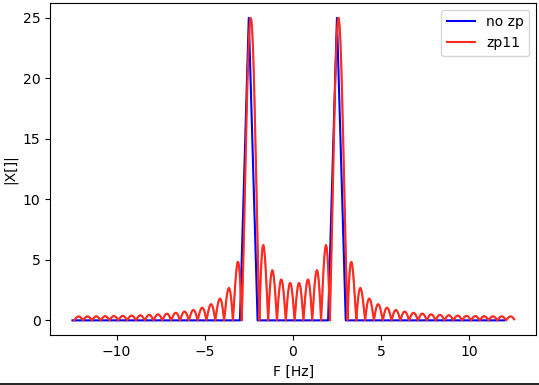
\includegraphics[width=\textwidth]{code/stft_harm_2.png}
    \end{minipage}
    \codecaption{dsv/code/stft_harm.py}{Einfluss der Fensterbreite bei der Analyse von harmonischen Schwingungen}\label{py:stft_harm}
\end{listing}
%
%
\clearpage
Man kann sich diesen Effekt aber auch zunutze machen und somit das Ergebnis der \gls{dft} beeinflussen, indem man das Signal vor der \gls{dft} noch zusätzlich fenstert, wobei man die Fensterfunktion genau so konzipiert, wie man es gerne hätte\linkfootnote{{https://docs.scipy.org/doc/scipy/reference/signal.windows.html}}.

Wenn wir uns beispielsweise an die Diskussion bezüglich der möglichen Dynamik in einem Signal erinnern, so kann es sein, dass man eher an Dynamik als an Auflösung interessiert ist.
In solch einem Fall, kann man beispielsweise auf ein Hann-Fenster\linkfootnote{{https://docs.scipy.org/doc/scipy/reference/generated/scipy.signal.windows.hann.html}} zurückgreifen und anstatt einem Vektor $\bm x$ transformieren wir mit der \gls{dft} den Vektor $\bm w \odot \bm x$, wobei $\odot$ die punktweise Multiplikation repräsentiert.
Dies führt dazu, dass wir im Frequenzbereich eine Faltung mit der \gls{dft} von $\bm w$ erhalten anstatt einem $\Sinc$.

In \Cref{py:stft_win} sehen wir nun, dass dies erlaubt Frequenzanteile zu finden, die sich ohne explizite Fensterung in den sogenannten Nebenwellen der $\Sinc$-Funktion \q{verstecken}.
Die Nebenwellen der $\Sinc$-Funktion fallen ab gemäß
\[
\Abs{\Sinc(x)} \leqslant \frac{1}{x},
\]
wobei andere Fensterfunktionen im Frequenzbereich deutlich schneller abfallen können.
Wir sehen aber auch, dass sich hier wiederum ein Trade-Off aufzeigt, da die sogenannte Hauptkeule der \gls{dft} von $\bm w$ deutlich breiter ist als die der $\Sinc$-Funktion.
Das heißt, dass man durch Auswahl der Fensterfunktion zwischen Auflösung im Sinne von $\Delta_{1,2}$ und Dynamikbereich wählen kann, beziehungsweise \emph{muss}.
Denn, wie wir gesehen haben, impliziert eine \gls{dft} \emph{immer} eine Multiplikation mit der entsprechenden $\Rect$-Funktion und man kann diese nur gegen eine andere ersetzen, aber nicht vermeiden!
Für die \gls{stft} bedeutet dies, dass wir hier mit derselben Fragestellung konfrontiert sind und entsprechend den Anforderungen der speziellen Anwendung wählen müssen.

\begin{listing}[ht]
    \noindent
    \begin{minipage}{0.51\textwidth}
        \strut\vspace*{-\baselineskip}\newline
        \inputminted[firstline=5, lastline=22]{python3}{code/stft_win.py}
    \end{minipage}%
    \begin{minipage}{0.48\textwidth}
        \strut\vspace*{-\baselineskip}\newline
        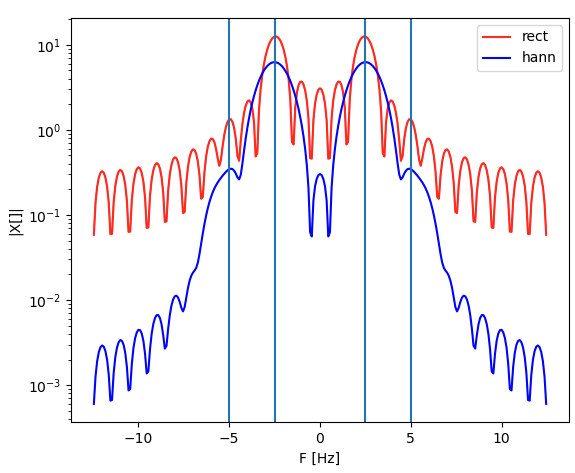
\includegraphics[width=\textwidth]{code/stft_win.png}
    \end{minipage}
    \codecaption{dsv/code/stft_win.py}{Geschickte Fensterung kann den Dynamikbereich erhöhen}\label{py:stft_win}
\end{listing}
%
%
\clearpage
Als nächstes wollen wir mit \Cref{py:stft_length} den Punkt machen, dass bei der \gls{stft} direkt Auflösung im Frequenzbereich gegen Auflösung im Zeitbereich getauscht wird.
Wollen wir Änderungen im Frequenzbereich präzise in der Zeit verorten, brauchen wir entsprechend kurze Fenster, doch opfern dafür Genauigkeit bei der Bestimmung des eigentlichen Frequenzwertes.
Andererseits können wir ein Signal länger, mit einem breiten Fenster, beobachten und dann haben sehr gute Auflösung im Frequenzbereich, was aber impliziert, dass wir nicht genau sagen können, \emph{wann} sich Dinge im Frequenzbereich ändern.

\begin{listing}[ht]
    \noindent
    \begin{minipage}{0.51\textwidth}
        \strut\vspace*{-\baselineskip}\newline
        \inputminted[firstline=5, lastline=30]{python3}{code/stft_length.py}
    \end{minipage}%
    \begin{minipage}{0.48\textwidth}
        \strut\vspace*{-\baselineskip}\newline
        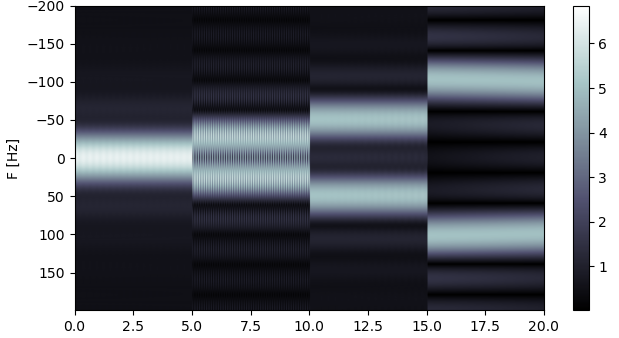
\includegraphics[width=\textwidth]{code/stft_length_1.png}\\
        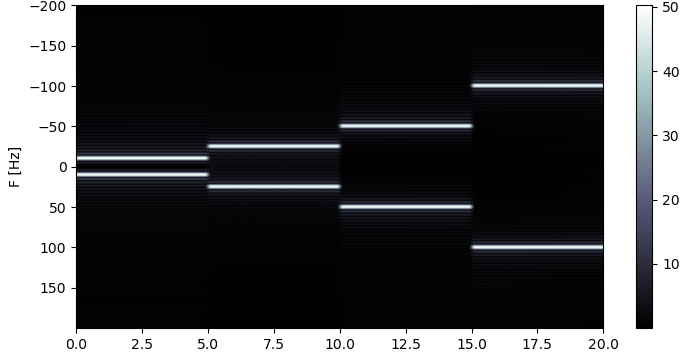
\includegraphics[width=\textwidth]{code/stft_length_2.png}\\
        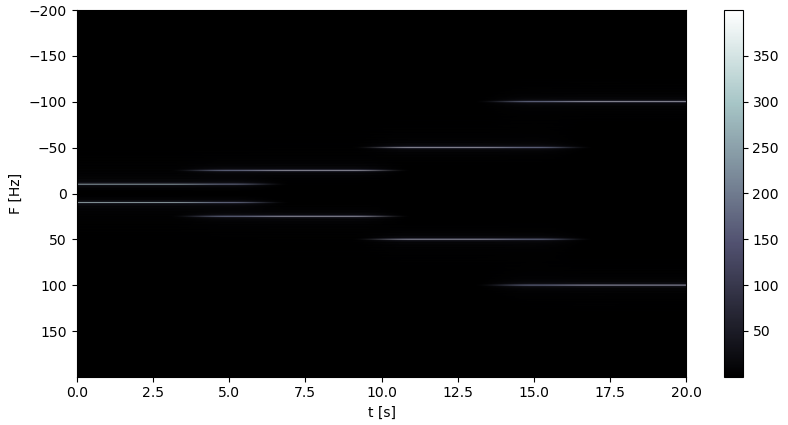
\includegraphics[width=\textwidth]{code/stft_length_3.png}
    \end{minipage}
    \codecaption{dsv/code/stft_length.py}{\acrshort*{stft} für verschiedene Fensterlängen}\label{py:stft_length}
\end{listing}
%
\clearpage

Als letztes wollen wir ein Beispiel für eine Anwendung der \gls{stft} zeigen. 
In \cref{py:stft_bass} wurde mit einer Bassgitarre eine G-Dur-Tonleiter eingespielt und in entsprechende Blöcke zerteilt, die in etwa den einzelnen Tönen entsprechen.
Im Frequenzbereich wurde dann eine \q{peak search} genutzt, um die lokalen Maxima der einzelnen \gls{dft}-Blöcke zu finden.
Die ermittelten Frequenzen der einzelnen Töne passen sehr gut zu denen, die man online in Tabellen\linkfootnote{{https://mixbutton.com/mixing-articles/music-note-to-frequency-chart/}} finden kann.
\begin{listing}[ht]
    \noindent
    \begin{minipage}{0.51\textwidth}
        \strut\vspace*{-\baselineskip}\newline
        \inputminted[firstline=10, lastline=44]{python3}{code/stft_bass.py}
    \end{minipage}%
    \begin{minipage}{0.48\textwidth}
        \strut\vspace*{-\baselineskip}\newline
        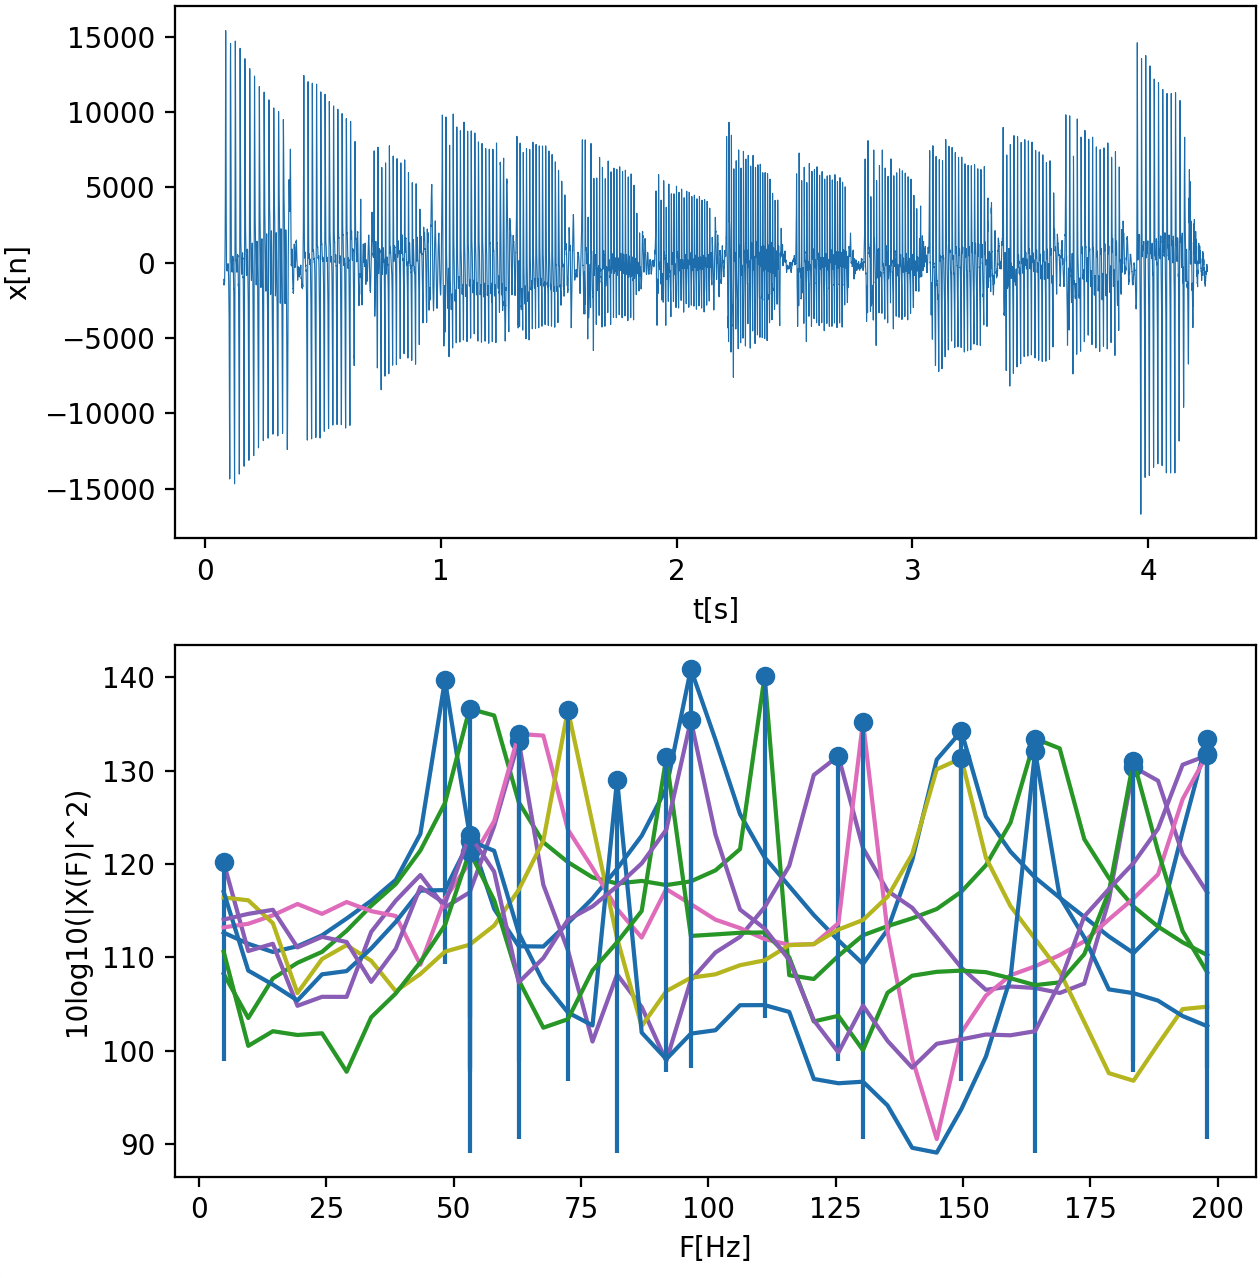
\includegraphics[width=\textwidth]{code/stft_bass.png}\\
    \begin{minted}{python}
    [ 48.2811  96.5622 149.6715 197.9527]
    [ 53.109  111.0466 164.1559]
    [  4.8281  62.7654 125.5309 183.4683]
    [ 62.7654 130.3590 197.9527]
    [ 72.4217 149.6715]
    [ 53.109   82.0779 164.1559]
    [ 53.109   91.7341 183.4683]
    [ 53.109   96.5622 197.95270418]
    \end{minted}
    \end{minipage}
    \codecaption{dsv/code/stft_1.py}{Analyse einer \q{Bassline} mittels \acrshort*{stft}, die eine G-Dur-Tonleiter spielt}\label{py:stft_bass}
\end{listing}

